Due to the mechanism of kinetic mixing, the production of the heavy photon is similar to that of a photon radiating from an electron although at a suppressed rate proportional to the coupling $\epsilon^2$. The final states into which the heavy photon can decay is related to the model of the dark sector and corresponding dark matter mass $m_{\chi}$. A heavy photon that is heavier than $2m_{\chi}$ can decay into completely invisible states or a mixture of invisible states and SM states. Here, we focus solely on the scenario of a heavy photon that decays visibly to SM particles (this also implies that the heavy photon is lighter than twice the lightest dark matter mass). 

\subsection{Decay signature}
The branching ratio of the heavy photon is obtained from the ratios of different final state measurements of $e^+e^-\rightarrow $ hadrons at various center-of-mass energies~\cite{liu_signals_2015}. In the mass regime that HPS explores, the heavy photon will decay to $e^+e^-$ pairs as shown in Figure~\ref{Figure:br}. 

\begin{figure}[htb]
  \centering
      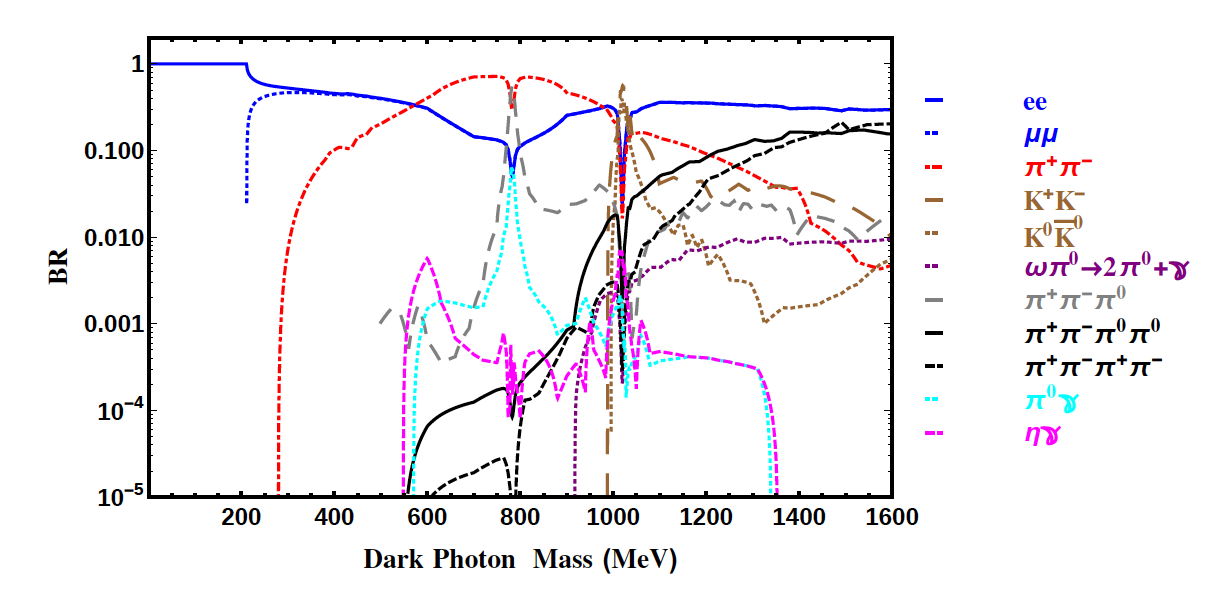
\includegraphics[width=0.9\textwidth]{pics/motivation/branchingRatio.png}
 	 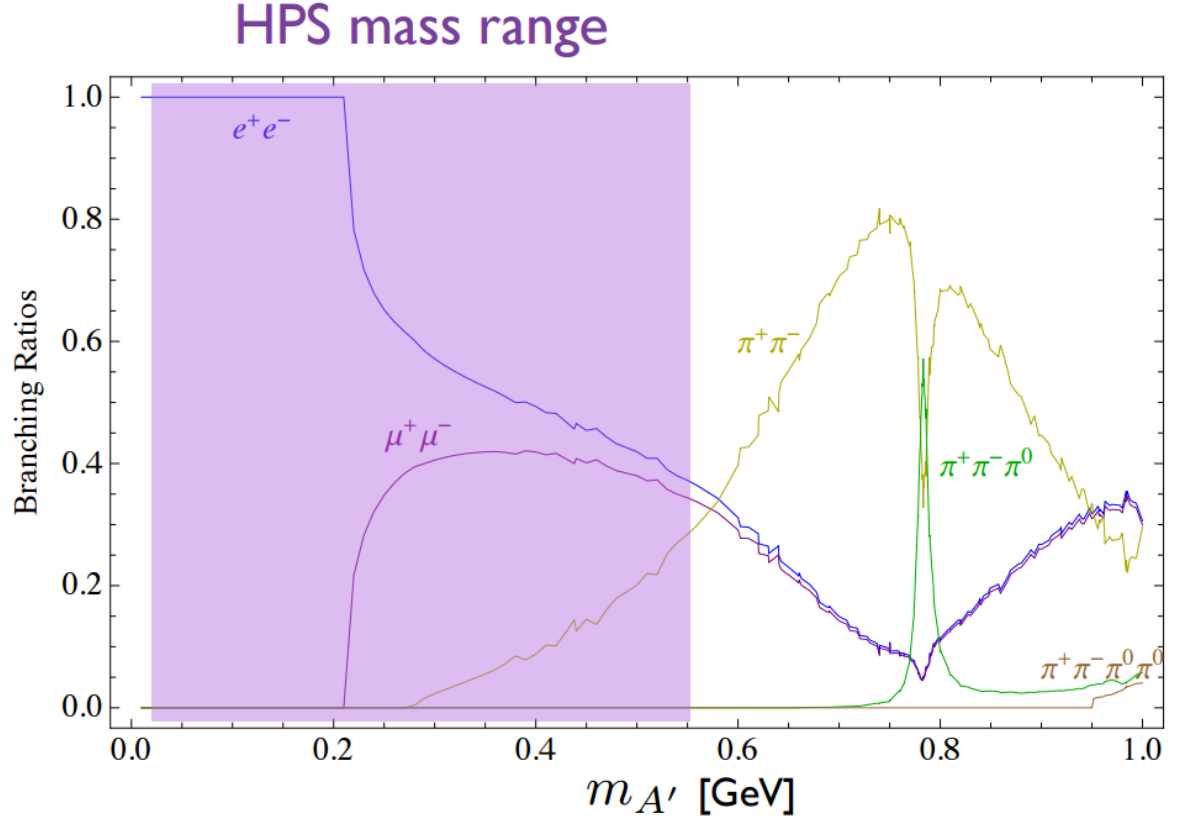
\includegraphics[width=0.5\textwidth]{pics/motivation/branchingLinear.png}	
  \caption[The branching fraction ratios for heavy photon decays]{The branching fraction ratios for heavy photons of various masses is shown~\cite{liu_signals_2015}. The mass range that HPS is most sensitive to is highlighted in the bottom plot.}
  \label{Figure:br}
\end{figure}

HPS searches for heavy photons of masses 20 to 100~MeV/c$^2$. As shown in Figure~\ref{Figure:br}, at heavy photon masses above 200~MeV/c$^2$, the branching ratio for decays to $e^+e^-$ begins to decrease sharply and the turn on for decays to $\mu^+\mu^-$ becomes significant. \\
\indent Assuming that the heavy photon only decays to SM final states, the proper lifetime of the $A^{\prime}$ neglecting phase space corrections is described by Equation~\eqref{eq:propLife} where $N_{eff}$ is the number of available decay states ($=1$ at $m_{A^{\prime}}<2m_{\mu}$)~\cite{bjorken_new_2009}. 

\begin{equation}
	\label{eq:propLife}
	\begin{split}
	c\tau &= \dfrac{1}{\Gamma}\simeq \dfrac{3}{N_{eff}m_{A^{\prime}}\alpha\epsilon^2}\\
	&\simeq \dfrac{0.8\textrm{ cm}}{N_{eff}}\Big({\dfrac{10^{-4}}{\epsilon}}\Big)^2\Big(\dfrac{100\textrm{ MeV}}{m_{A^{\prime}}}\Big)
	\end{split}
\end{equation}

The lifetime is inversely proportional to the coupling $\epsilon^2$. For small couplings, the heavy photon will travel a measurable distance before decaying. The decay length is 

\begin{equation}
	\label{eq:decayL}
	\begin{split}
	l_0 &\equiv \gamma c \tau \\
	&\simeq \dfrac{0.8\textrm{ cm}}{N_{eff}}\Big(\dfrac{E_{beam}}{10\textrm{ GeV}}\Big)\Big({\dfrac{10^{-4}}{\epsilon}}\Big)^2\Big(\dfrac{100\textrm{ MeV}}{m_{A^{\prime}}}\Big)^2
	\end{split}
\end{equation}

where $E_{beam}$ is the incident electron energy. The rate of $A^{\prime}$ production is dependent on $\alpha^3\epsilon^2/m_{A^{\prime}}^2$ and is suppressed relative to ordinary bremsstrahlung by a factor of $\epsilon^2m_{e-}^2/m_{A^{\prime}}^2$~\cite{bjorken_new_2009}. The ratio of the fully differential production cross sections for the heavy photon relative to the production of a virtual photon are described in Equation~\eqref{eq:production}.

\begin{equation}
	\label{eq:production}
	\dfrac{d\sigma(e^-Z\rightarrow e^-ZA^{\prime}\rightarrow e^-Zl^+l^-)}{d\sigma(e^-Z\rightarrow e^-Z\gamma^{\ast}\rightarrow e^-Zl^+l^-)} = \Big(\dfrac{3\pi\epsilon^2}{2N_{eff}\alpha}\Big) \Big(\dfrac{m_{A^{\prime}}}{\delta m_{A^{\prime}}}\Big)
\end{equation}

This ratio represents the maximum signal to background that can be achieved in an experiment. The heavy photon is produced at very forward, small angles and carries nearly all of the beam energy. \\

\subsection{Methods of production}
Heavy photons can be produced experimentally in fixed-target experiments and collider experiments. Fixed-target experiments are complementary to collider experiments in that they can generally access smaller coupling due to the high luminosity while collider experiments can probe higher heavy photon masses due to the higher center of mass energy attainable. In electron fixed-target experiments, the heavy photon is generated through a bremsstrahlung-like process and is detected from the final state particles. Proton fixed-target experiments look for the signal in the decay products of various meson decay channels produced from the beam interaction at the target. Looking for heavy photons produced in meson decays such as Dalitz decays ($\pi^0, \eta, \eta^{\prime}\rightarrow \gamma A^{\prime}$), ($K\rightarrow\pi A^{\prime} $, $\phi\rightarrow\eta A^{\prime}$, and $D^{\ast}\rightarrow D^{0}A^{\prime}$) are another production mechanism that has been used at both colliders and fixed target-type experiments. Drell-Yan ($q\bar{q}\rightarrow A^{\prime}$) experiments are more common at proton fixed target and hadron collider experiments. Both $e^+e^-$ colliders and hadron colliders search from heavy photons in the decay channels listed above and are particularly well-suited to search for heavy photons that decay invisibly due to the ability to precisely reconstruct the initial state. 

\subsection{Methods of detection}

The strategies for searching for heavy photons are typically a bump hunt on the visible final state particles, a bump hunt in the missing mass spectrum (assumes that the heavy photon does not decay visibly), or a detached vertex search for heavy photons with small couplings. \\
\indent Electron fixed target experiments produce heavy photons through bremsstrahlung-like processes with the electron beam incident on a heavy target. Heavy photons are produced in a very forward direction requiring high resolution spectrometers or detectors close to the beam. Previous limits set by this type of experiment include the A1 experiment that uses the Microtron beam at Mainz and the A1 high resolution spectrometer to reconstruct $e+e-$ pair~\cite{beranek_theoretical_2013}. The A1 significantly ruled out parameter space where the heavy photon was a possible explanation to resolve the muon $g-2$ anomaly. The APEX experiment at Jefferson Lab ran a test run experiment that produced electron bremsstrahlung in Hall A and used the high resolution spectrometers to measure the $e^+e^-$ particles~\cite{abrahamyan_search_2011}. APEX performed a bump hunt on the final state particles in the mass range 65-600~MeV and will likely take data again in 2018. DarkLight is another Jefferson Lab experiment that places a windowless gas target in the Low Energy Recirculator Facility using a 100~MeV beam to search for heavy photons with low masses. DarkLight will perform a bump hunt search in the $e^+e^-$ mass spectrum and may have some ability to search for invisible decays by using a silicon layer to detect proton recoils~\cite{alewski_darklight_2014}.\\
\indent Proton fixed target experiments look for heavy photons in the decays of particles produced from beam interaction at the target. The NA48/2 experiment at the CERN SPS produced $K^{\pm}$ beams and searches for heavy photons from the $\pi^0$ decay produced from in the in-flight decay of the $K^{\pm}$~\cite{Batley_2015lha}. SHiP is future experiment at the CERN SPS that will use a 400~GeV proton beam and will look in both Drell Yan and meson decays for heavy photons. SHiP will be sensitive to long decay lengths (on the order of 10s of meters) and will cover a wide mass range in visible decay states up to 10~GeV masses. SHiP is expected to run sometime after 2026~\cite{ship_collaboration_facility_2015}.\\
\indent Beam dump experiments look for heavy photons with long decay lengths. The beam dump experiments E141 and E137 at SLAC, E774 at Fermilab, and one at Orsay were originally run to look for MeV-mass axion-type particles from electron beam dumps~\cite{alexander_dark_2016}. The U70 beam dump looked for heavy photons downstream from a proton beam on a fixed target. SeaQuest at Fermilab looks for muon pairs produced downstream from the 120~GeV proton beam on a fixed target. It is speculated that by analyzing previous data taken (E906/SeaQuest), a 95$\%$ confidence limit on heavy photon masses in the range of 215-5600~MeV is possible. SeaQuest is currently establishing upgrades for improved future running~\cite{gardner_new_2016}.
\indent Collider experiments using $e^+e^-$ or proton collisions complement the fixed-target experiments and are favored for looking for heavy photon invisible decays.  BaBar, an experiment at the Stanford Linear Accelerator (SLAC) $e^+e^-$ collider, set limits by searching for the $A^{\prime}$ in missing mass around the $\Upsilon(2S)$, $\Upsilon(3S)$, and $\Upsilon(4S)$ resonances~\cite{Lees_2014xha}. In the near future, LHCb at CERN is expected to look for heavy photons in the di-muon invariant mass spectrum from rare heavy quark decays produced from proton-proton collisions. LHCb will be sensitive to the heavy photons with both prompt and displaced vertices and is expected to run sometime after 2021~\cite{Ilten_2016tkc}.